\documentclass[a4paper]{article}
\usepackage{amsmath, amssymb, textcomp}
\usepackage{graphicx}
\usepackage{cite}
\usepackage[hidelinks]{hyperref}
\usepackage[section]{placeins}
\usepackage[font=footnotesize,labelfont=bf]{caption}
\newcommand{\Part}[3][ ]{\ensuremath{\frac{\partial^{#1} #2}{{\partial #3}^{#1}}}}
\newcommand{\Dif}[3][ ]{\ensuremath{\frac{d^{#1} #2}{{d #3}^{#1}}}}
\renewcommand{\O}[1]{\ensuremath{\mathcal{O}\left(#1\right)}}
\renewcommand{\vec}{\bold}

\begin{document}
\title{Plasma Analysis}
\author{Tobias de Jong \& David Kok}
\date{\today}
\maketitle

\section{Introduction}
%{\bf Fysische achtergrond, motivatie voor numeriek. Bonuspunten voor gebruik van het woord Topologisch }
In this project we will numerically determine some topological properties of magnetic field lines in a plasma.
The numerical computations involved are heavily parallelizable. 
For this reason computations are done on a GPU, which can run thousands threads in parallel, instead of the CPU which on modern computers can only run $\sim$10 parallel processes.
We use CUDA to write code to efficiently calculate the topological properties of magnetic field lines as generated in recent full-magnetohydrodynamical numerical studies of magnetic reconnection.~\cite{PhysRevLett.115.095001}

This work concentrates on plasmas in which the field lines have a non-trivial topological order, such as interlocking rings. 
As linking is a conserved quantity in MHD, this topological order enhances the stability of the plasma.

The studied system consists of the evolution through time of the plasma, with an initial configuration of two or more interlocked rings. These rings evolve into a set of nested tori.
In this work we will compute topological properties of these tori, foremost the winding number.

To implement the code we were inspired by Marek Fiser.\footnote{\url{http://www.marekfiser.com/Projects/Real-time-visualization-of-3D-vector-field-with-CUDA}} He uses Runge-Kutta integration to visualize (air) flows around a Delta wing, but the idea of integration of a vector field is the same.

\section{Theory and Methods}
\subsection{Theory of field lines}
We want to calculate properties of the magnetic field, using the field lines associated to the field. In order to do this we need (finite segments of) field lines. To describe these field lines it is sufficient to note that field lines are the solutions $\vec x(s)$ to the following ordinary differential equation:
\[\Dif{\vec x}{s} = \vec B(\vec x),\]
where $s$ is the parametrization variable.\\
An interesting observation made by \cite{taylor1986relaxation} is that in an ideal plasma the total helicity of the field $H_{\text m}$, defined through the volume integral:
\[
	H_{\text m} = \int\vec{A}\cdot\vec{B}\ d\vec{x} = \int\vec{A}\cdot (\nabla\times\vec{A})d\vec{x}
\]
is conserved. Therefore the initial value of this integral restricts the possible long-term dynamics of a plasma. 

In particular we are working with a dataset of highly helical initial data, in which case the field lines will align themselves along the surfaces of nested tori. 
A line on the surface of a torus can be associated with a winding number, which is the ratio of the winding along the toroidal axis (denoted with $\alpha$) and the winding along the poloidal axis (denoted $\beta$). 
To calculate a field line and its winding numbers we will use numerical integration as described in more detail below.


\subsection{Methods}
To compute the properties of interest we use a CUDA program.\footnote{Full code available on Github: \url{https://github.com/TAdeJong/plasma-analysis}}.
Our code is split into two main segments. 

Firstly we numerically integrate the magnetic field to obtain an approximation of a field line in the plasma. 
Secondly we compute several properties of the magnetic field using this field line, such as the length of the line (which estimates the average field strength), the center of the line (estimating the origin of the torus on which it lies) and its winding number, i.e. its contribution to the total helicity of the magnetic field.

Both steps can be parallelized heavily. To parallelize the numerical integration of the magnetic field we simply consider more than one field line at a time. 
In the second step we not only consider multiple field lines at once, but also parallelize the computation of the aforementioned parameters per field line.

Both the fact that we need to calculate many field lines and the fact that all field lines are independent, with almost no conditional steps in the property calculation, indicate that a GPU will be a powerful instrument to tackle this problem.


\section{Numerical Aspects}
\subsection{Vector field representation}
Note that we are interested in the field lines for fixed moments in time, so all our analysis will not take into account any time evolution of the plasma. 
Thus the magnetic field is a pure 3D vector field $\vec{B}: \mathbb{R}^3 \to \mathbb{R}^3$. To represent this field in a computer a discretization is needed. 
This is done by defining a rectangular grid in space and saving the components of the field at each grid point. 

There are two ways to save all the components: either separate the components and save a three-dimensional array for each component of the vector field (three $N\times N\times N$ arrays), or save one large array of which each component contains the whole vector at the corresponding gridpoint (one $N\times N\times N$ array of $3D$ vectors).

Since numerical integration algorithms will use all the components of the field at a point at the same time we use the second method. %Or do we? Ik weet eigenlijk niet hoe een 3D texture van binnen werkt...
This choice of representation is both physically intuitive as well as efficient, since it will improve cache coherency and therefore access times.

\subsubsection{Interpolation}
In order to accurately integrate we need accurate estimates of the original vector field at arbitrary locations. 
It is unfeasable to have a discretization fine enough such that we have a value for each location of interest. 
We therefore want to interpolate the vector field to get a good approximation of the value of the vector field at an arbitrary location.
The simplest method for interpolation is linear interpolation, for 3D data known as trilinear interpolation.

Interpolation of two- and even three-dimensional data is used in graphics processing in order to map images onto three-dimensional objects. 
In GPU-parlance this is known as texturing. Because this problem is very important in graphics processing, modern GPU's have efficient texturing units, performing hardware accelerated trilinear interpolation.

Using CUDA enables us to use this hardware accelerated interpolation by storing our vector field data as a texture. 
Since every RK4-step needs at least 4 vector field fetches this acceleration significantly speeds up the numerical integration. %alhoewel we dit natuurlijk niet gemeten hebben.

\subsection{Runge-Kutta method}
For line integration the fourth order Runge-Kutta method (RK4) was used.  This method is known as a good allround integration method.
Compared to standard Forward Euler, RK4 uses four values of the magnetic field to calculate the next point on the field line. 
This increase in calculation time per step is compensated by a vastly reduced error per step, allowing for a much larger step size $\Delta s$, since RK4 has a much higher order total accumulated error $\O{\Delta s^4}$.

\section{Algorithm}
At a high level our algorithm consists of three steps: 
\begin{enumerate}
	\item Calculate the field line
	\item Determine a toroidal coordinate system for this field line
	\item Calculate the required properties in this new coordinate system
\end{enumerate}
We will further eleborate on these steps below and comment on the complexity.\\

\subsection{Step by step}

To calculate the winding number of a field line passing through a certain starting point we first use RK4 to integrate a length of field line from the magnetic field data. This length should be large enough such that we have a high number of revolutions around the torus.

This integration process is inherently sequential, i.e. computations on later RK4-steps can not be performed before the results from all earlier steps have been computed, leaving no room for parallelization on a per step basis.
Due to the hardware optimized interpolation we are memory access bound in this part of the algorithm, which we have verified by using the NVIDIA profiler. 
Thus there was nothing to be gained from parallelizing the integration further than one-thread-per-field-line.

\begin{figure}[!htb]
\minipage{0.45\textwidth}
  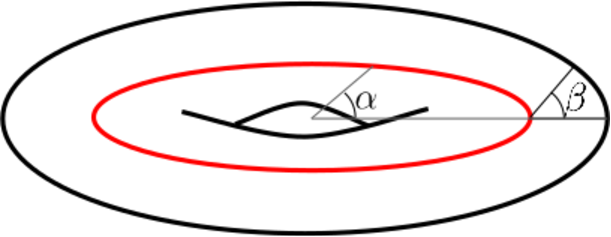
\includegraphics[width=\linewidth]{Figures/TorusAlphaBeta.pdf}
\endminipage\hfill
\minipage{0.45\textwidth}
  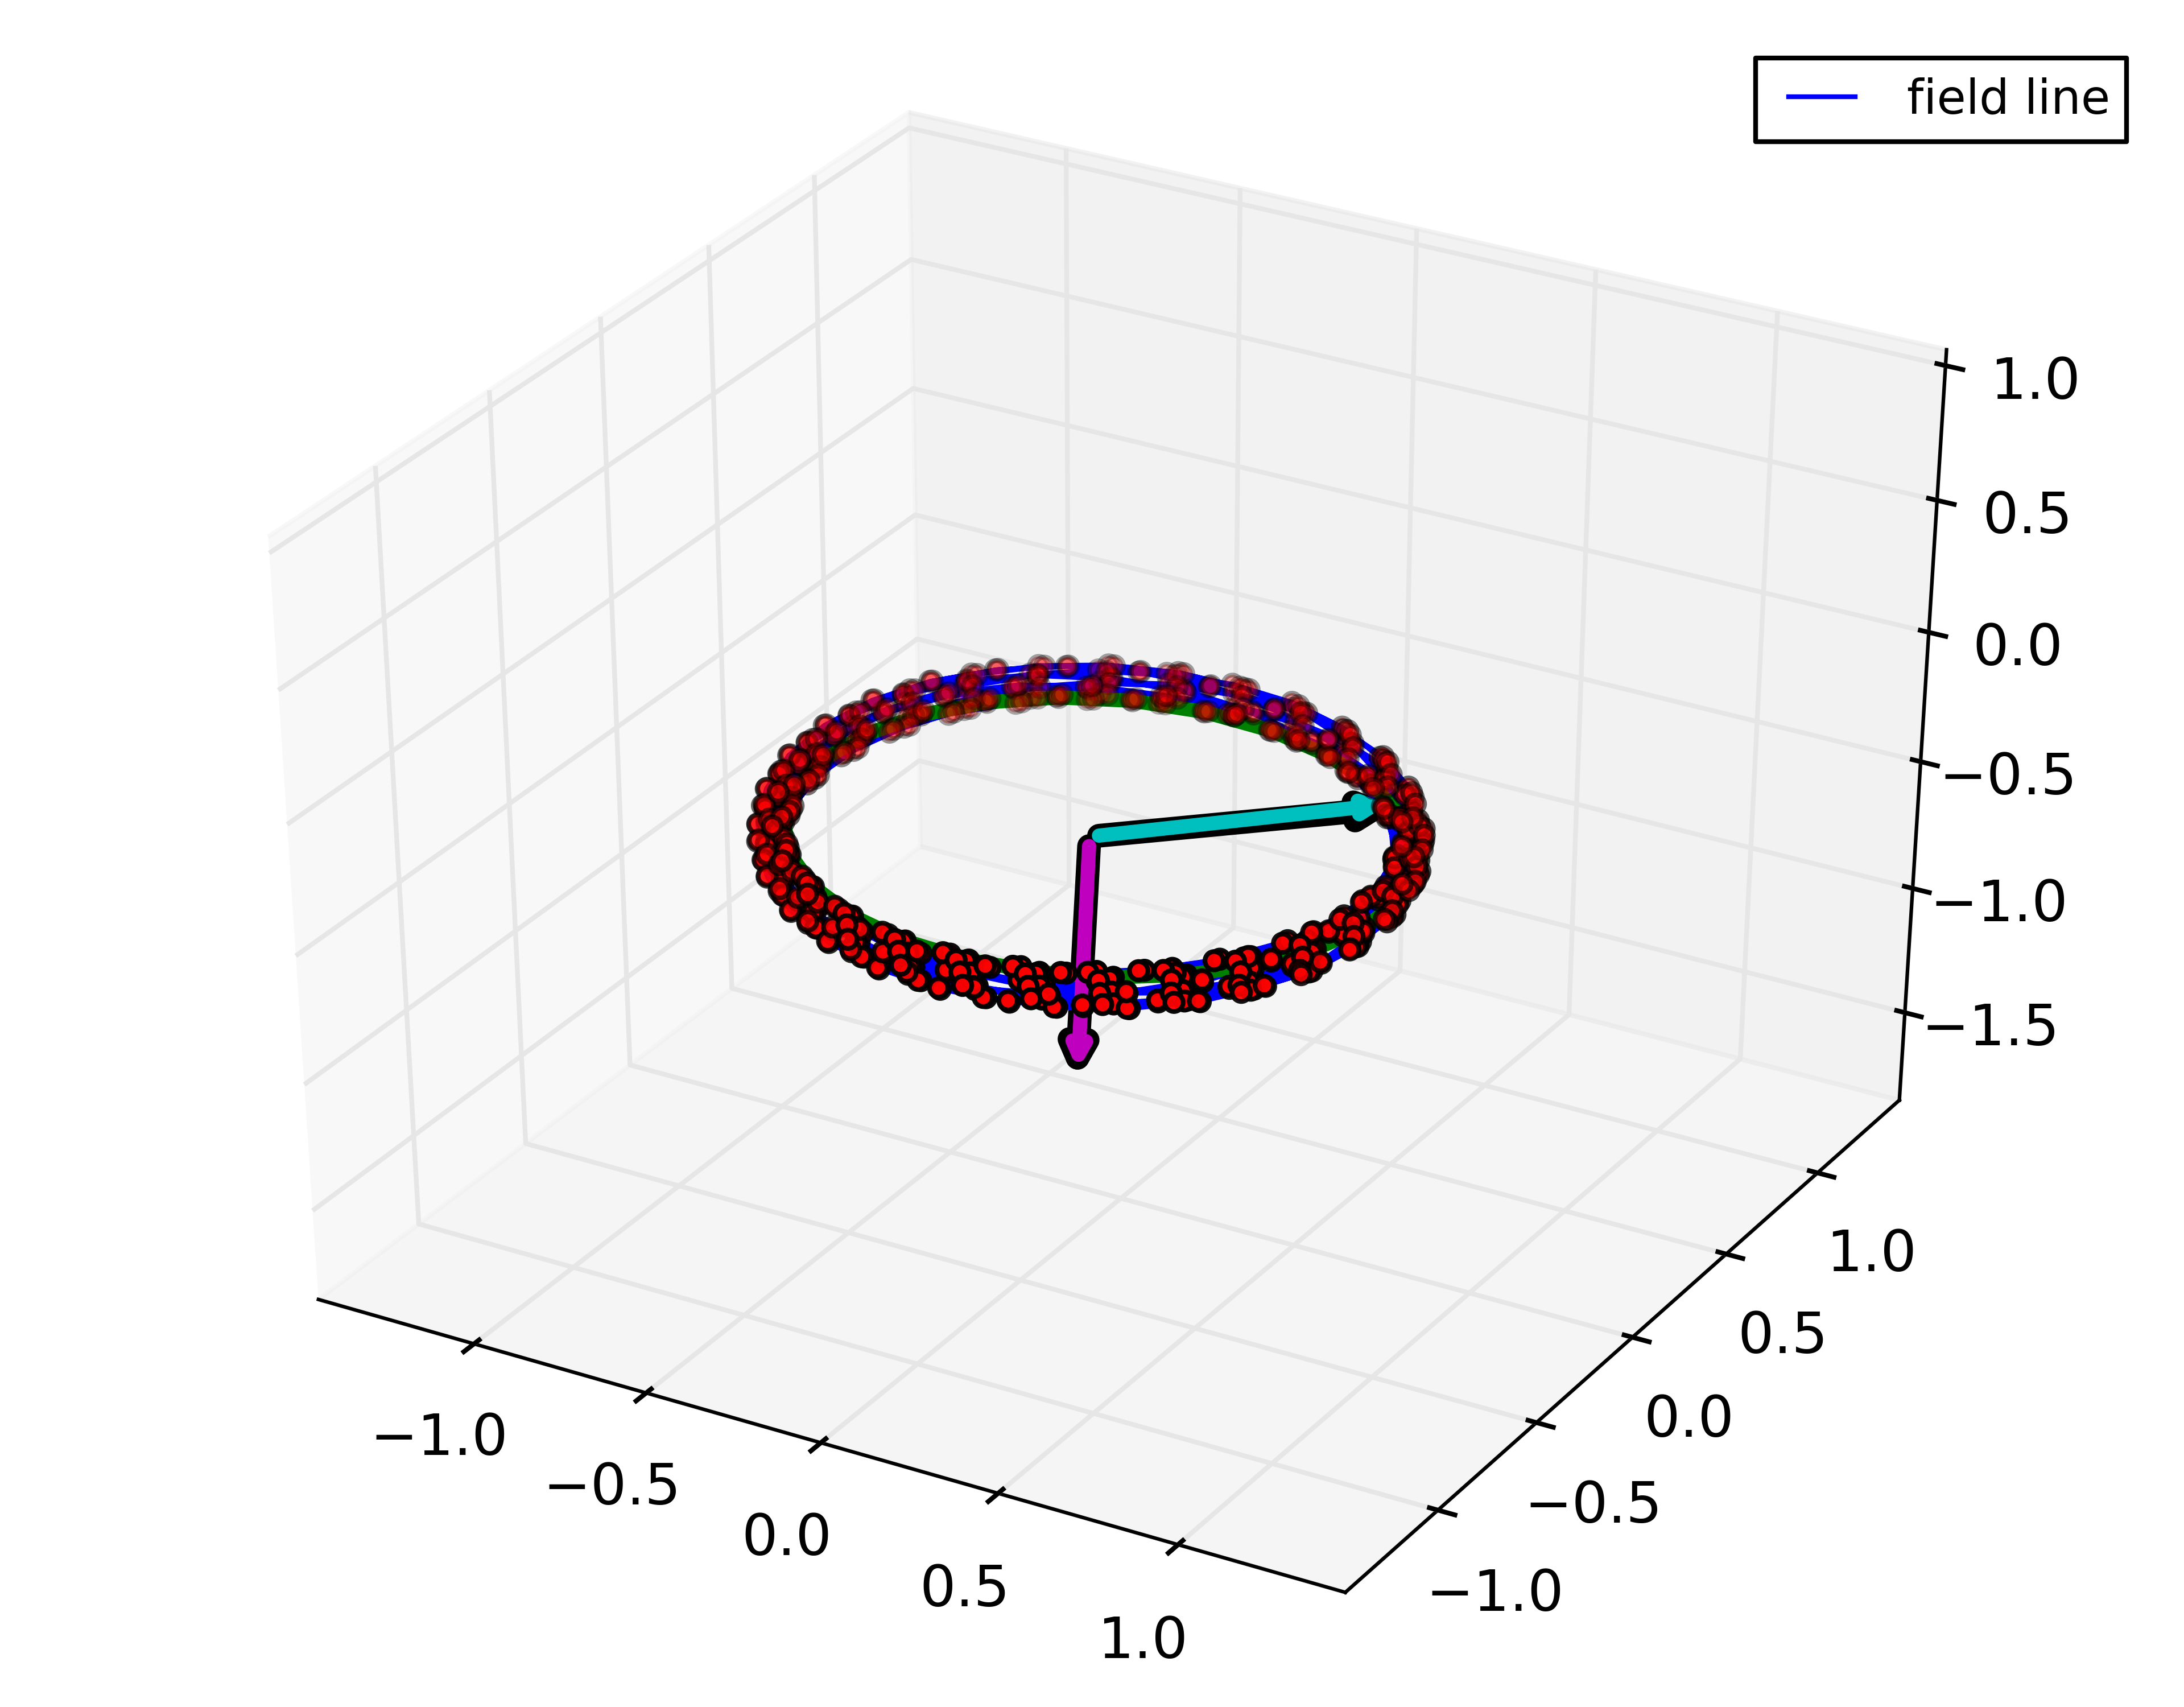
\includegraphics[width=\linewidth]{Figures/torusfit3.png}
\endminipage
	\caption{Illustration of the toroidal coordinate system and the normal finding procedure.}\label{fig:coordsys}
\end{figure}

To compute the winding number of a field line we need to convert to a toroidal coordinate system. Since not all tori of interest are perfectly aligned this means we first have to find the position and orientation of the torus of interest before we can calculate any other relevant parameters.

By averaging the coordinates over a whole field line we find (a good approximation of) the origin of our torus. This summation can be done efficiently in parallel as a reduction. For implementation we implemented most of the methods described by Harris et al.~\cite{harris2007optimizing}.

Next we need to calculate the orientation of the torus, in particular the normal to the surface plane of the torus. 
We can find this normal by taking the cross product of the direction of a field line (the $\vec{B}$-field) at a point and the location vector of that point. We perform this local calculation for each point on our field line and implement a similar parallel reduction as before to find the orientation of our torus.

The last part of the torus coordinate system needed is the (center) radius of the torus. For this we calculate the average distance from the origin in the projection onto the plane of the torus. %This is error prone, see discussion.

With this coordinate system calculating the winding numbers of the field lines is as simple as calculating the difference in both poloidal and toroidal coordinates between consecutive data points and summing these along a field line. This is once again implemented as a parallel reduction.

In the implementation it was needed to take care of unwrapping the coordinates modulo $2\pi$ using some inefficient if-statements. %Discussion: One could probably devise a parallel unwrap algorithm, but would it be worth it?
As a last step, the ratio of the total polodoidal and toroidal change is computed to find the winding number.

As mentioned before this entire algorithm is parallelized by considering multiple field lines simultaneously. In particular we pick a 2D-grid of initial locations for the field lines instead of a single point. Using this data we can show the winding number as a function of position in the nested tori.\\
\subsection{Complexity}
In order to analyse the theoretical (time) complexity let's introduce the following variables:
\begin{itemize}
	\item $p$, the maximum number of concurrent threads on the GPU
	\item $m$, the number of RK4-steps per field line.
	\item $N$, the number of pixels in our picture, equal to the total number of field lines calculated.
\end{itemize}
As is clear from the definitions, the time needed for the integration will be linear in $m$. As soon as the number of field lines is larger than the number of threads, a linear factor in $N/p$ comes in as well, as we have to divide the calculations over several rounds of computation:
\[t_{RK4}\in\O{m\left\lceil\tfrac{N}{p}\right\rceil}\]
For the reduction of a calculated value along a field line, we need $\frac m2$ threads. The reduction itself is logarithmic, so we have the following complexity:
\[t_\textit{reduc} \in \O{\left\lceil\frac{Nm}{2p}\right\rceil\log\left(m\right)} \]
Note that this is theoretically slower than performing a serial reduction per field line for a large enough number of field lines ( which would again have $t \in \O{\left\lceil N/p\right\rceil m}$ ), but cache locality and coherency favor this algorithm heavily.

Any local operations on datapoints of field lines are of course linear in the number of datapoints $mN$ and, as they are local (i.e. fully parallelizable), reduced by a factor of $p$.\\
On top of all this we expect our code to have a fixed contribution to the runtime from allocating memory, loading the magnetic field and initialising the hardware accellerated structures. We therefore expect the runtime of our code to be approximately linear in the numbers $m$ and $N$, but we do not expect this linear dependence to go through the origin.

\section{Results}
%{\bf plaatjes, timings + scaling, portability, meer plaatjes: lines, lengths, windings, masking}
\subsection{Simulated field lines}
Using our code we computed magnetic field lines for given magnetic fields. Included are three examples of the winding numbers computed with this code, and one example of the computed line lengths.


\begin{figure}[!htb]
\minipage{0.49\textwidth}
  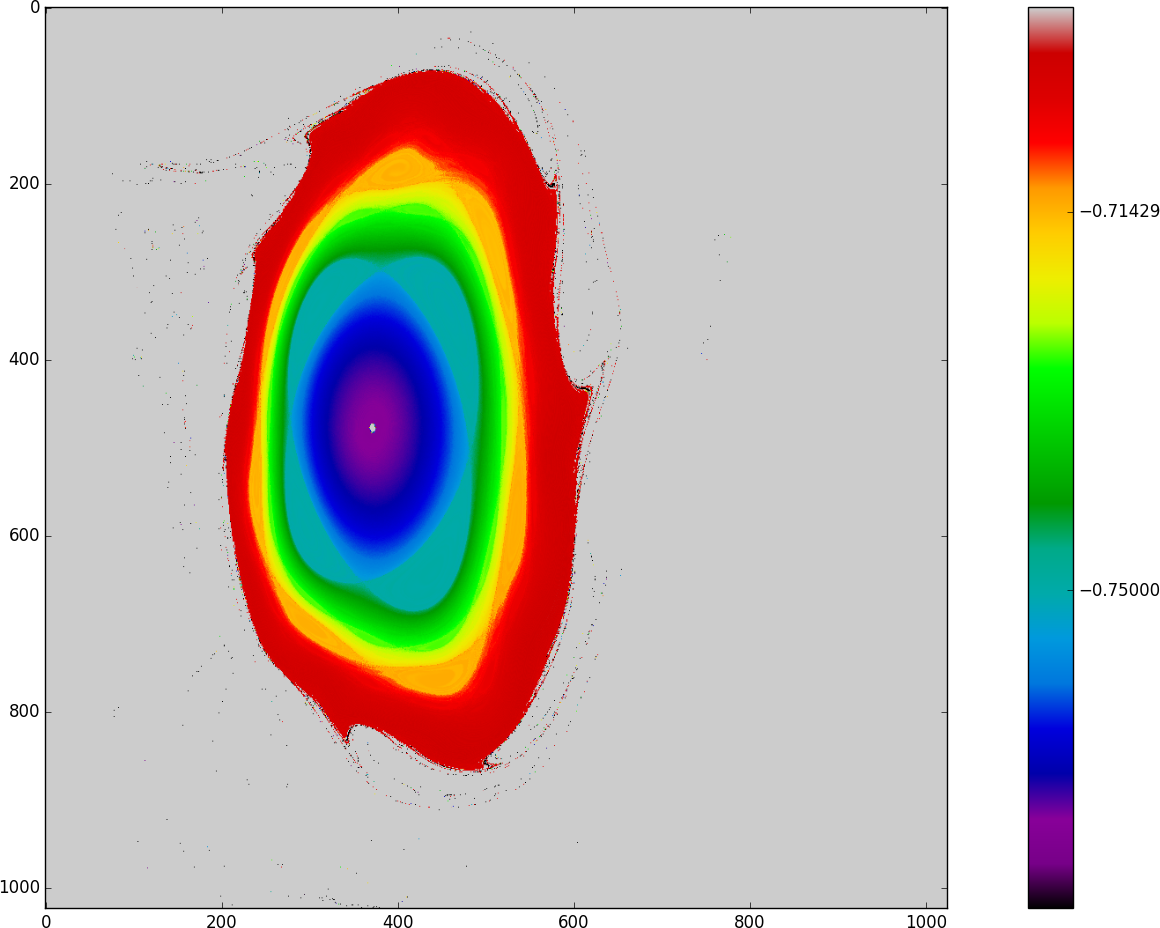
\includegraphics[width=\linewidth]{Figures/Rings_Papertwist_twist1_82_steps32k.png}
\endminipage\hfill
\minipage{0.49\textwidth}
  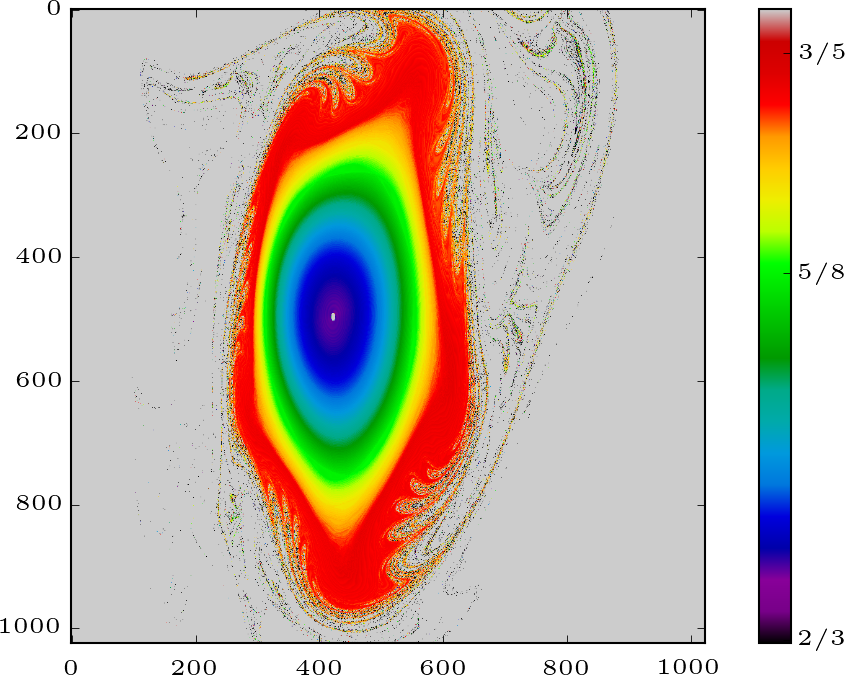
\includegraphics[width=\linewidth]{Figures/Rings_Papertwist_twist1_125_steps32k.png}
\endminipage
	\caption{Winding numbers of the field lines of a cross-section through the torus for the dataset \texttt{Papertwist1}. The color scale was cut on both sides to optimize for the structure inside the Torus. Both images have a resolution of $1024\times 1024$ pixels and use $32768$ points per field line. The left image is at time $t=82$, the right one at $t=125$.}\label{fig:125-32k}\label{fig:82-32k}
\end{figure}

In order to make a good image the data is restricted in two ways. 
We firstly changed the colour scale to ensure that the changes in the nearly-constant winding number are visible. 
Secondly we have discarded (masked) all points with a total length of the field line below a certain threshold, reasoning that the winding numbers of short field lines can be wildly inaccurate. 
In this category fall nearly all field lines that leave the simulation box, as the texture clamps all vector field accesses to zero outside it.
For completeness we include a plot of the length of the field lines and the unmasked (but still colour-clipped) data in Figure \ref{fig:125-32k} below.\\

\begin{figure}[!hb]
\minipage{0.32\textwidth}
  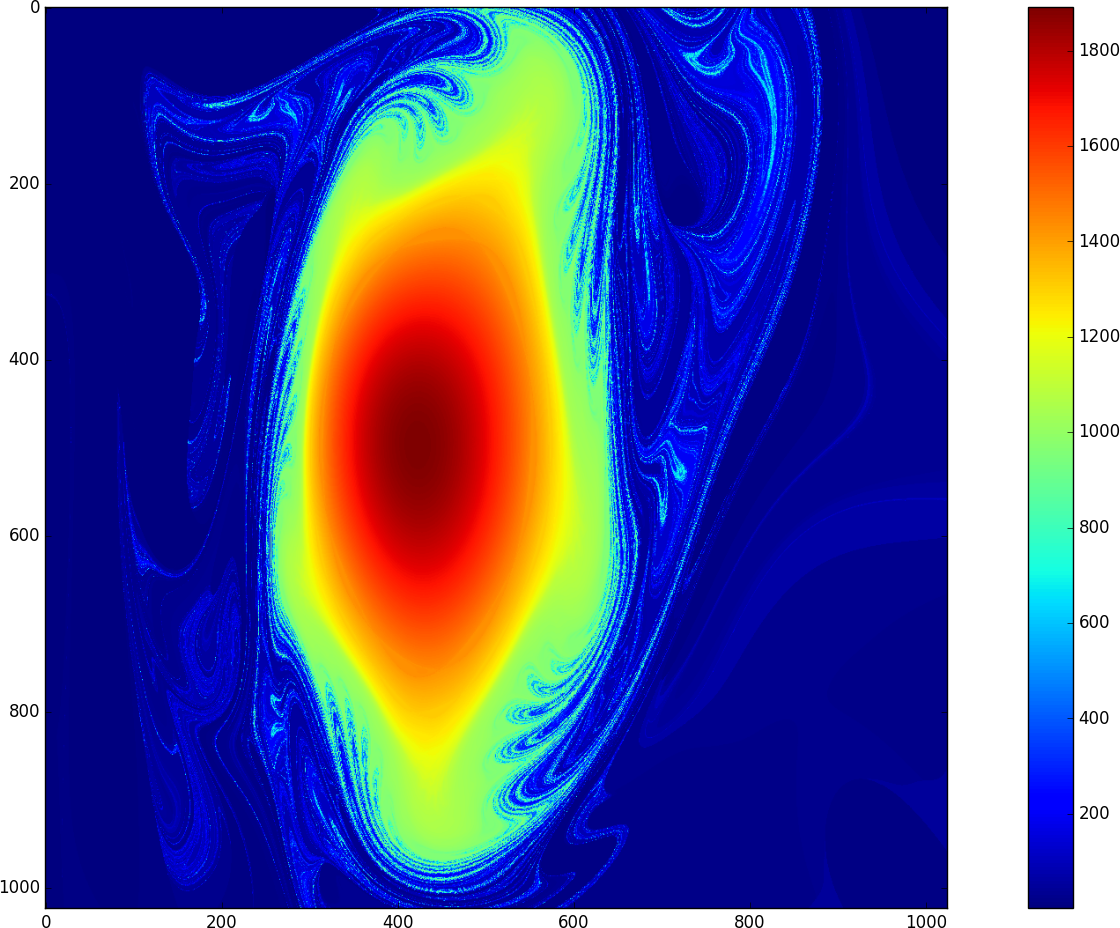
\includegraphics[width=\linewidth]{Figures/Rings_Papertwist_twist1_125_lengths_steps32k.png}
	\caption{Lengths of the field lines of a cross-section through the torus. The vector field used is \texttt{Papertwist1-125}. The image is $1024\times 1024$ pixels, with $32768$ points per field line.}\label{fig:125-lengths}
\endminipage\hfill
\minipage{0.32\textwidth}
  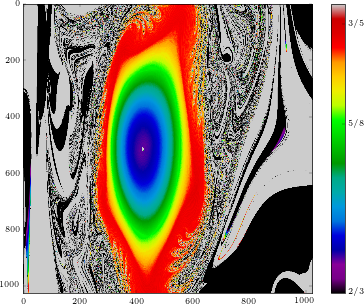
\includegraphics[width=\linewidth]{Figures/Rings_Papertwist_twist1_125_nomask_steps32k.png}
	\caption{Unmasked winding numbers of the field lines of a cross-section through the torus. The vector field used is \texttt{Papertwist1-125}. The image is $1024\times 1024$ pixels, with $32768$ points per field line.}\label{fig:125-unmasked}
\endminipage\hfill
\minipage{0.32\textwidth}
  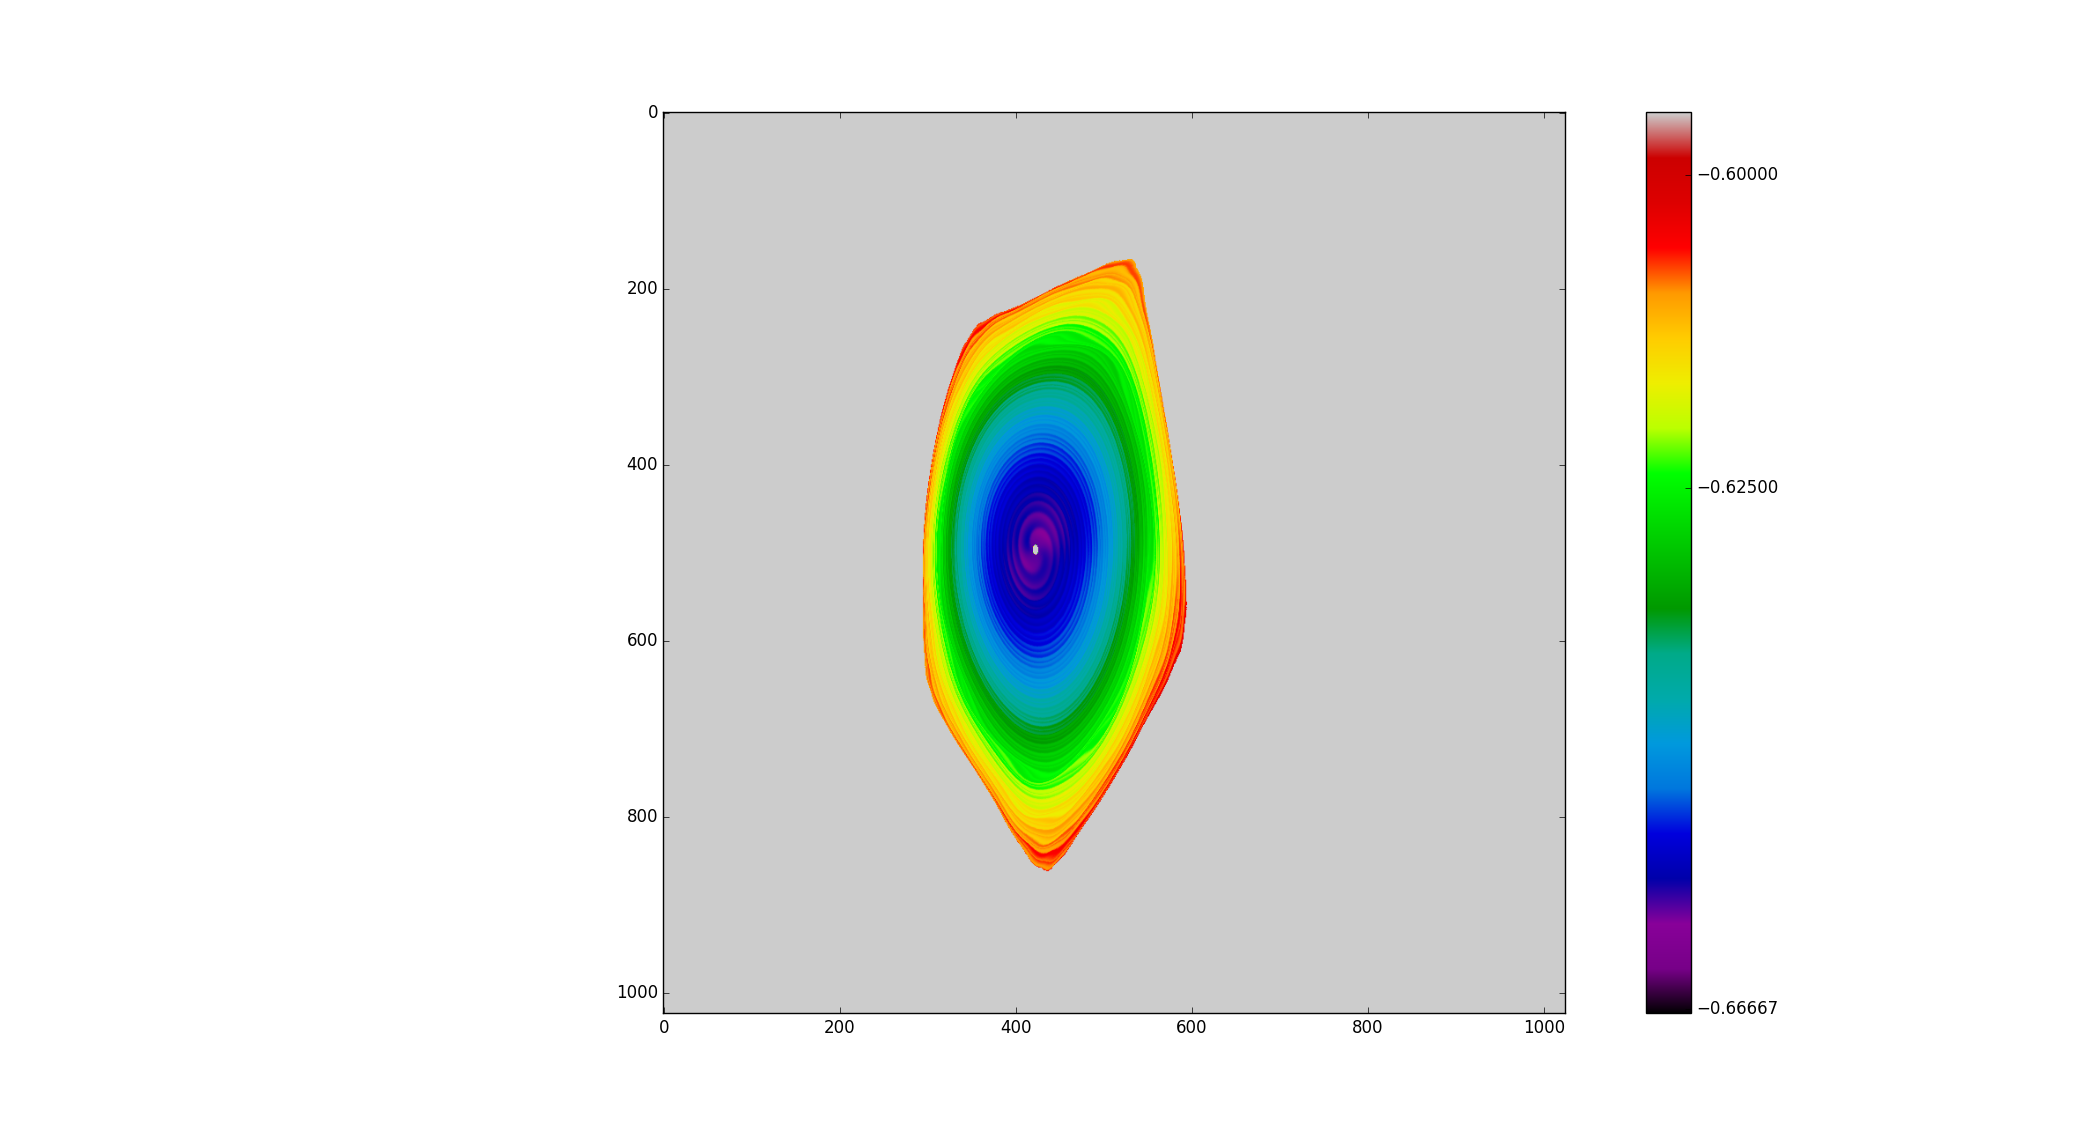
\includegraphics[width=\linewidth]{Figures/Rings_Papertwist_twist1_125_steps8k.png}
	\caption{Identical to Figure~\ref{fig:125-32k}, albeit with $8196$ points per field line. Although most of the features reproduce, numerical `ripples' arise due to the too short integration time, as dicussed in Section \ref{section:numerrors}.}\label{fig:125-8k}
\endminipage
\end{figure}

\FloatBarrier
\subsection{Speed and scaling}
We have recorded the runtime of the code on a NVIDIA GTX1080 for the dataset \texttt{Shafranov\_Rot3\_ampl\_0.05\_Animation50}, generating and analysing datasets as in Figure \ref{fig:82-32k}. For the first set of timing data we fixed the image size at $1024\times 1024$ pixels (field lines) and varied the number of steps per field line. After that we fixed the number of steps per field line (at $32768$) and varied the number of pixels in an image.\\
\begin{figure}[!ht]
	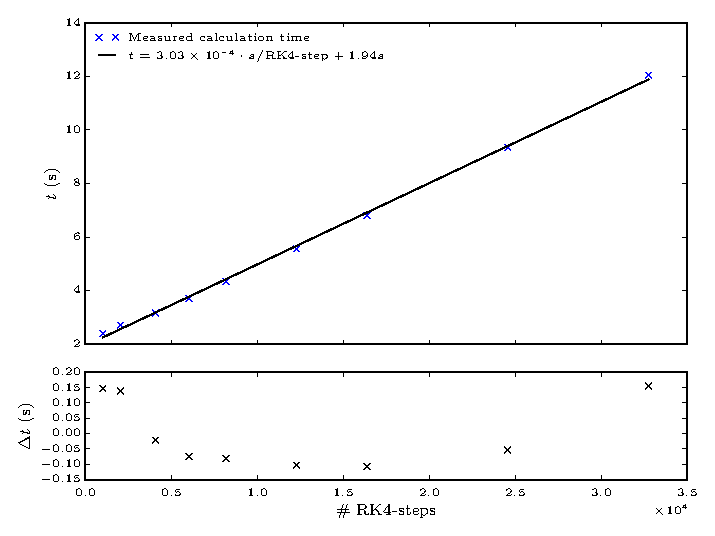
\includegraphics{Figures/timings_1.pdf}
	\caption{Linear fit of the computation time as a function of the number of RK4-steps, with the deviation from the fit plotted below. This was done for a resolution of $1024 \times 1024$}\label{fig:timings1}
\end{figure}
\begin{figure}[!ht]
	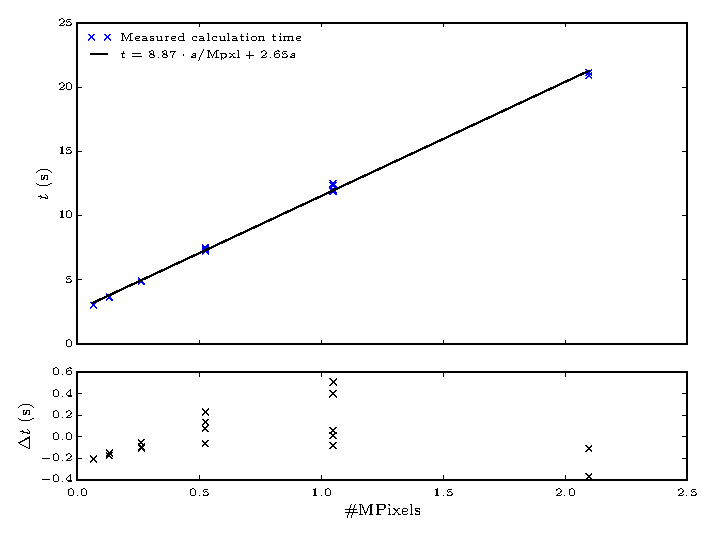
\includegraphics{Figures/timings_2.pdf}
	\caption{Linear fit of the computation time as a function of number of field lines for 32768 RK4-steps each, with the deviation from the fit plotted below.}\label{fig:timings2}
\end{figure}

%\FloatBarrier

We compare the performance of our program with the prevous method used, which also computed winding numbers for plasma field lines.
This existing Python code simulated a $1\times 1100$ array of field lines with 4000--16000 RK6-steps per line, and took approximately $36$ hours for this computation. 
Comparing this with our own results we conclude that our program is faster by a factor of approximately $3.5\cdot 10^6$.\\

Lastly we used the NVIDIA visual profiler to see how much memory our code was using while active. 
While generating a $1024\times 1024$ dataset with $32768$ steps per field line the program was using $6513$ MiB while in use, whereas running the code with identical parameters except for halving the number of steps per line (to $16384$) the program was using $3441$ MiB.


\section{Discussion}
In this section we interpret the results of our code, and suggest possible improvements. 
In particular we discuss the accuracy of the used method for calculating the magnetic structure and how numerical errors effect the computed structure.

\subsection{Numerical errors}\label{section:numerrors}
There are two features in the results that merit further discussion. 

\subsubsection{Coordinate system inaccuracy}

\begin{figure}[!hb]
	\centering
	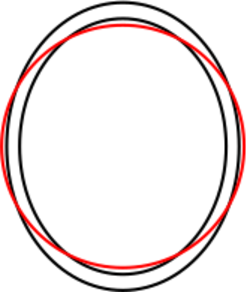
\includegraphics{Figures/TorusMismatch.pdf}
	\caption{ Illustration of the coordinate system mismatch between the calculated torus centre (red) and actual, elliptical, torus.}\label{fig:mismatch}
\end{figure}
Firstly we remark that near the center of each of the cross-sections the winding numbers behave oddly (the small white dots in the centers of Figure \ref{fig:82-32k}).
Closer inspection reveals that there is a sign flip in the winding number of the field lines here, which shows up as white due to the colour scale. 

We suspect that this sign flip is due to a numerical error in the code, possibly caused by the change in coordinate systems. 
Since our transformation of Cartesian coordinates to Toroidal coordinates is based on the line data, this coordinate change is likely to be inaccurate for small tori. 
In particular we determine a radius of- and normal to- a circle around the origin of a field line, and assume that this circle lies inside the torus on which the field line lies. If this circle intersects a cross-section of the torus near the edge of the cross-section all results based on the toroidal coordinate system will contain a small error (whereas it would be perfect if they intersect in the centre of the cross section). 
If this intersection instead happens outside the torus we can safely say that all winding numbers computed in the toroidal coordinate system are useless. 

Since in practice the tori on which the field lines lie may be elliptical (instead of perfectly circular), the only way to completely avoid this error may be through more thorough analysis of these surfaces.\\

\subsubsection{Finite length}
Secondly it is interesting to consider the differences between Figure \ref{fig:125-8k} and Figure \ref{fig:125-32k}, in particular the apparent shapes near the center of the cross section, reproduced in Figure \ref{fig:artefacts}.
\begin{figure}[!hb]
	\centering
\minipage{0.42\textwidth}
  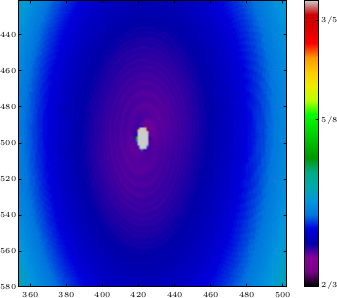
\includegraphics[width=\linewidth]{Figures/artefact32k.png}
\endminipage ~
\minipage{0.42\textwidth}
  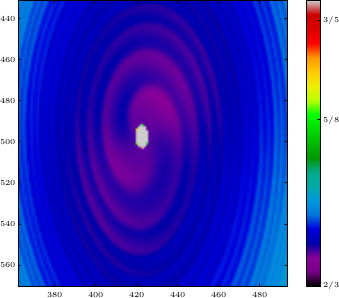
\includegraphics[width=\linewidth]{Figures/artefact8k.png}
\endminipage\hfill
	\caption{Zoom of Figures \ref{fig:125-32k} and \ref{fig:125-8k}, corresponding to 32k RK4-steps and 8k RK4-steps.}\label{fig:artefacts}
\end{figure}


In Figure \ref{fig:125-8k} we clearly see shapes with twofold rotational symmetry around the white center, which are much less pronounced and different in shape in Figure \ref{fig:125-32k}.
We suspect that these patterns in the winding numbers may be due to the finite length of the simulated field lines. 

As mentioned above, the surfaces on which our field lines lie are not perfect tori but rather are slightly elliptical. This implies there are sections of field line where the local winding number is not equal to the global (average) winding number along a line. 
Therefore after a finite number of data points the average of our simulated line may disagree with the true winding number (corresponding to an infinitely long line). 
This problem is made far worse by the fact that our toroidal coordinate system is not optimized for correcting this eccentricity, which explains why these features are most prominent at the center of the cross section. 

A possible solution might be to use a more sophisticated method to extract the winding number from the local data than the (weighed) average that is currently in place, although it should be noted that most of these methods are hard to parallellize and will therefore significantly slow down the algorithm.\\

We would furthermore like to remark that, as always when numerically integrating a vector field, there is a tradeoff between small step size (and low truncation error in the numberical method) and large step size (and low total number of steps for fixed length, so a low cumulative rounding error). 
In our code we fix the step size inversely proportional to the average magnitude of the magnetic field in the dataset. 
Therefore the spatial step size, with a length of our step size times the local magnitude of the magnetic field, is on average constant between different input fields. 
A possible improvement on this would be to dynamically scale the step size at each integration step, ensuring that all spatial steps taken are of very similar length. Regular adaptive step size algorithms however branch depending on whether a step was determined to be too large or too small, making them ill-fitted for the SIMT (Single Instruction Multiple Threads) parallelism of GPU's.\\

\subsection{Speed and scaling}
We note that the memory usage agrees well with our theoretical predictions, where we consider that we store (for the $32768$ steps per line):
\begin{itemize}
	\item The vector field, $256\times256\times256$ \texttt{Float4} objects ($16$ Byte each), for a total of $256$ MiB.
\item The line data itself, $64\times 64$ lines (this part of the code is serialized so not all lines need to be stored at the same time) times $32768$ \texttt{Float4} points per line, for a total of $2048$ MiB.
\item One array to compute and store the normal vectors to the tori of interest, which needs to be of the same size as the line data array, so $2048$ MiB total.
\item Two scalar fields to compute and store the toroidal and poloidal windings of $64\times 64\times 32768$ Floats, which equals $512$ MiB per field or $1024$ MiB total.
\item One scalar field to compute and store the length of the vector fields, for $512$ MiB total.
\item One scalar field to compute and store the middle radius of the tori, for $512$ MiB total.
\end{itemize}
In total this adds up to $6400$ MiB, which is in good agreement with the observed $6513$ MiB. 
To find the theoretical memory use for the simulation with $16384$ steps per field line we repeat the calculation above and find a total of $3328$ MiB in theory, which agrees well with the $3441$ MiB observed. 
In both cases we are using $113$ MiB more than was predicted in theory, which we attribute to general overhead.\\

Secondly we observe that, as was predicted, the runtime of our code is highly linear in both the number of pixels/field lines and the number of steps per field line, with an offset of about two seconds. 
We conclude that this is the amount of time that it takes to load the vector field to the memory on the graphics card and allocate all relevant arrays (the two different datasets above give a different time offset because they correspond to different array sizes that need to be allocated), and that the complexity of the algorithm is as predicted.

\section{Suggestions for future work}

\subsection{Interpolation}
Better algorithms exist for interpolation, most notably cubic interpolation and interpolation schemes which preserve the zero divergence of the magnetic field~\cite{McNally01052011}. It is possible that these algorithms could further reduce numerical artefacts. 
Notably, efficient and open source implementations in CUDA of cubic interpolation exist~\cite{Ruijters01012012}.

\subsection{Integration}
As mentioned the code was shown to be largely memory access bound. Implementation of a multi-step method such as Adams-Bashforth could reduce the number of texture fetches per step, while maintaining a high order.\\
Also worth mentioning is that the RK4 integration method uses no special properties of the magentic field, such as the divergencelessness or the Hamiltonian description. It might for example be possible to exploit the knowledge that the system is Hamiltonian by implementing a symplectic method.

\subsection{Optimization}
Because the numerical integration is the only inherently sequential part of the algorithm, we made the choice to minimize calculations during this part of the algorithm. 
Profiling of the code shows however that it is both memory bound and memory access bound. 

A possible optimization would be to increase the computational load during the integration of the magnetic field, for example pre-calculating some of the properties required later, thus improving use of the other computational resources and overall efficiency during this part of the algorithm.

Another optimization opportunity is the memory usage. In the current code a lot of memory is used for computing the normal vectors and scalar fields. Efficient reuse of memory could reduce total memory usage per field line, enabling more field lines to be treated in parallel.



\newpage
\bibliographystyle{plain}
\bibliography{introduction}
\end{document}
